\section{Standard di qualità}
\subsection{ISO/IEC 12207}
ISO/IEC 12207 è uno standard ISO per la gestione del ciclo di vita del software.\\
\begin{figure}[h!]
	\centering
	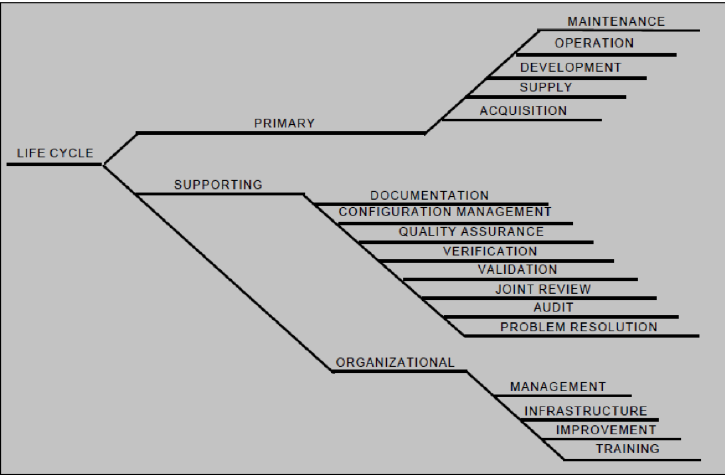
\includegraphics[scale=0.4]{res/images/ISO_12207.png}
	\caption{Processi del ciclo di vita del software, secondo lo standard ISO/IEC 25010:2011}
\end{figure}
Di tutti questi processi, elenchiamo quelli su cui ci siamo concentrati maggiormente.
\begin{itemize}
	\item Tra i \textit{processi primari}:
		\begin{itemize}
			\item \textbf{Sviluppo};
			\item \textbf{Fornitura}.
		\end{itemize}
	\item Tra i \textit{processi di supporto}:
		\begin{itemize}
			\item \textbf{Documentazione};
			\item \textbf{Gestione della configurazione};
			\item \textbf{Accertamento della qualità};
			\item \textbf{Verifica};
			\item \textbf{Validazione};
			\item \textbf{Risoluzione dei problemi}.
		\end{itemize}
	\item Tra i \textit{processi organizzativi}:
	\begin{itemize}
		\item \textbf{Gestione} (dei processi, comunicazione e rischi);
		\item \textbf{Infrastruttura}.
	\end{itemize}
\end{itemize}
\subsection{ISO/IEC 25010:2011}
In questo standard troviamo la parte di qualità del software, sostituisce l'ISO/IEC 9126 dal 2011 in poi.\\
In particolare aggiunge il modello della qualità in uso del software.\\
\begin{enumerate}
	\item \textbf{Efficacia:} precisione e completezza con cui gli utenti raggiungono i risultati desiderati.
	\item \textbf{Efficienza:} risorse spese in relazione agli obiettivi raggiunti (e in relazione all'efficacia).
	\item \textbf{Soddisfazione:} soddisfazione dell'utente, relativo ai suoi bisogni soddisfatti dal software.\\Solitamente la soddisfazione dipende dal soddisfacimento di \textit{utilità}, \textit{fiducia nel software}, \textit{gradimento} e \textit{comfort}.
	\item \textbf{Libertà da rischi:} grado con cui il software mitiga i possibili rischi.\\In particolare:
		\begin{itemize}
			\item mitigazione rischi economici;
			\item mitigazione rischi di salute e sicurezza;
			\item mitigazione rischi ambientali.
		\end{itemize}
	\item \textbf{Context coverage:} grado con cui il software può essere usato con efficacia\textsubscript{G}, efficienza\textsubscript{G}, soddisfazione e libertà da rischi, in qualunque contesto.
\end{enumerate}
Consultare la sezione ISO/IEC 9126 per altre informazioni sulla qualità del software.
\subsection{ISO/IEC 9126}
ISO/IEC 9126 è uno standard internazionale per valutare la qualità del software.\\
Questo standard fornisce un modello di qualità e 3 tipologie di metriche, queste 4 sezioni vengono riportate di seguito.\\
\begin{figure}[h!]
	\centering
	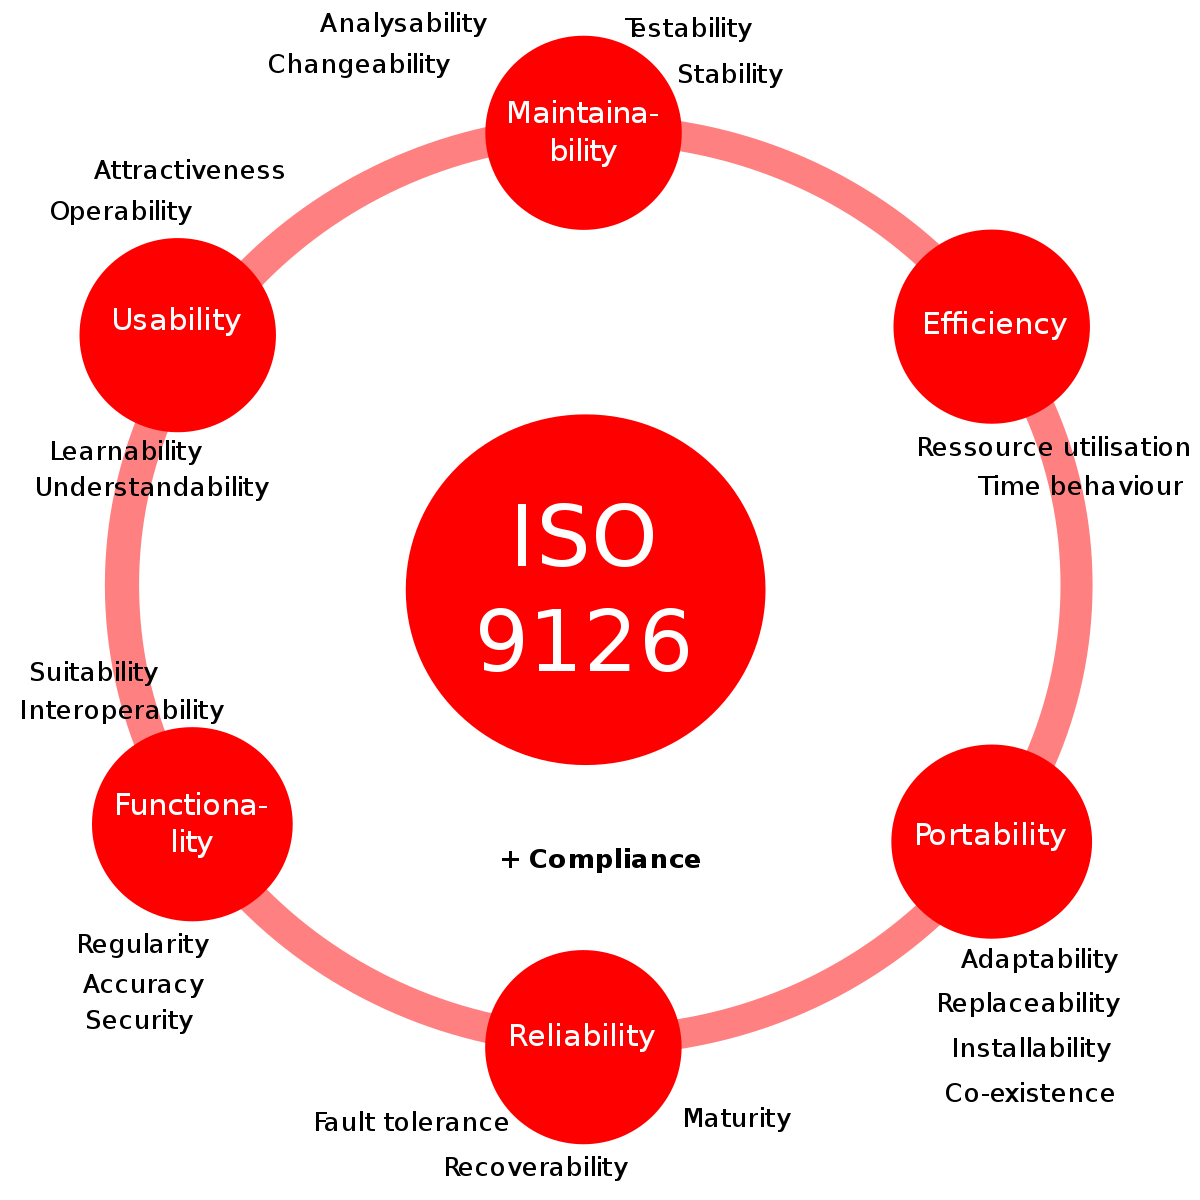
\includegraphics[scale=0.15]{res/images/ISO_9126.png}
	\caption{Figura esplicativa del modello della qualità software esterna ed interna dello standard ISO/IEC 9126}
\end{figure}
\subsubsection{Metriche per la qualità interna}
Definisce metriche applicabili al codice sorgente non eseguibile. Idealmente, la qualità interna determina la qualità esterna.\\
Viene rilevata tramite \textbf{analisi statica}.
\subsubsection{Metriche per la qualità esterna}
Definisce metriche applicabili al software in esecuzione che ne misurano i comportamenti tramite test. Idealmente, la qualità esterna determina la qualità in uso.\\
Viene rilevata tramite \textbf{analisi dinamica}.
\subsubsection{Metriche per la qualità in uso}
Definisce metriche applicabili solo quando il prodotto è finito e utilizzato in condizioni reali.
\subsubsection{Modello della qualità del software}
\begin{enumerate}
	\item \textbf{Funzionalità:} il software deve fornire funzioni che soddisfino i bisogni emersi nell'\textsc{Analisi dei Requisiti}.\\In particolare il software deve avere le seguenti caratteristiche:
		\begin{itemize}
			\item Appropriatezza;
			\item Accuratezza;
			\item Interoperabilità;
			\item Sicurezza.
		\end{itemize}
	\item \textbf{Affidabilità:} il software deve mantenere un certo livello di prestazioni quando utilizzato in condizione specificate.\\In particolare il software deve avere le seguenti caratteristiche:
		\begin{itemize}
			\item Maturità;
			\item Robustezza;
			\item Recuperabilità.
		\end{itemize}
	\item \textbf{Efficienza:} il software deve eseguire le proprie funzioni con minimo tempo e consumo di risorse possibile.\\In particolare efficienza\textsubscript{G} nel tempo, con veloci tempi di risposta e nello spazio, con una appropriata quantità di risorse.
	\item \textbf{Usabilità:} il software deve essere comprensibile e poter essere studiato senza troppe difficoltà.\\In particolare il software deve avere le seguenti caratteristiche:
		\begin{itemize}
			\item Comprensibilità;
			\item Apprendibilità;
			\item Operabilità;
			\item Attrattiva.
		\end{itemize}
	\item \textbf{Manutenibilità:} il software deve potersi evolvere con modifiche, correzioni e adattamenti.\\In particolare il software deve avere le seguenti caratteristiche:
		\begin{itemize}
			\item Analizzabilità;
			\item Modificabilità;
			\item Stabilità;
			\item Testabilità.
		\end{itemize}
	\item \textbf{Portabilità:} il software deve poter essere trasferito da un ambiente hardware/software ad un altro seguendo le evoluzioni tecnologiche.\\In particolare il software deve avere le seguenti caratteristiche:
		\begin{itemize}
			\item Adattabilità;
			\item Installabilità;
			\item Conformità;
			\item Sostituibilità.
		\end{itemize}
\end{enumerate}
